\documentclass[11pt,letterpaper,titlepage]{article}

\usepackage{geometry}
\geometry{left=2cm,right=2cm,top=2cm,bottom=3cm}

\usepackage{setspace}
\onehalfspacing

\usepackage{multicol}
\setlength{\columnsep}{3em}

\usepackage{booktabs}

\usepackage[table,x11names]{xcolor}

\usepackage{multirow}

\usepackage{pgfgantt}

\usepackage{listings}

\usepackage{xcolor}
\definecolor{vgreen}{RGB}{104,180,104}
\definecolor{vblue}{RGB}{49,49,255}
\definecolor{vorange}{RGB}{255,143,102}

\lstdefinestyle{C-style}
{
    language=C,
    basicstyle=\small\ttfamily,
    keywordstyle=\color{vblue},
    identifierstyle=\color{black},
    commentstyle=\color{vgreen},
    % numbers=left,
    numberstyle=\tiny\color{black},
    numbersep=11pt,
    tabsize=4,
    moredelim=*[s][\colorIndex]{[}{]},
    literate=*{:}{:}1
}

\lstdefinestyle{txt-style}
{
    basicstyle=\small\ttfamily,
    % numbers=left,
    numbersep=11pt,
    tabsize=4,
    moredelim=*[s][\colorIndex]{[}{]},
    literate=*{:}{:}1
}

\usepackage{tikz}
\usetikzlibrary{shapes.geometric, arrows, positioning, fit,calc}
\newcommand*\circled[1]{\tikz[baseline=(char.base)]{
            \node[shape=circle,draw,inner sep=1pt] (char) {#1};}}
            
\usepackage{hyperref}
\hypersetup{
    colorlinks,
    citecolor=black,
    filecolor=black,
    linkcolor=black,
    urlcolor=black
}

\usepackage{pifont}

\usepackage[toc,page]{appendix}

\pagestyle{empty}
\usepackage{tikz}
\usetikzlibrary{shapes.geometric, arrows}

\usetikzlibrary{mindmap,trees}
\usepackage{verbatim}

\usepackage{indentfirst}
\setlength{\parindent}{2em}

\usepackage{listings}

% \usepackage{hyperref}
\usepackage{chngcntr}
\counterwithin{section}{part}
\renewcommand\thesection{\arabic{section}}

\usepackage{graphicx}

\usepackage{subcaption}

\usepackage{fancyhdr}

\pagestyle{fancy}
\lhead{}
\rhead{}
\lfoot{ECEN 749 Section 601 Lab 2}
\cfoot{\thepage}
\rfoot{@Lei Wang (Wilson)}
\renewcommand{\headrulewidth}{0pt}
\renewcommand{\headwidth}{\textwidth}
\renewcommand{\footrulewidth}{0.4pt}
\newcommand{\RomanNumeralCaps}[1]
    {\MakeUppercase{\romannumeral #1}}

\makeatletter
\newcommand*\@lbracket{[}
\newcommand*\@rbracket{]}
\newcommand*\@colon{:}
\newcommand*\colorIndex{%
    \edef\@temp{\the\lst@token}%
    \ifx\@temp\@lbracket \color{black}%
    \else\ifx\@temp\@rbracket \color{black}%
    \else\ifx\@temp\@colon \color{black}%
    \else \color{vorange}%
    \fi\fi\fi
}
\makeatother

\usepackage{trace}

\begin{document}

\begin{titlepage}
  \centering
	{\scshape\large Texas A\&M University \par}
	\vspace{1cm}
	{\scshape\Large Department of Electrical and Computer Engineering \par}
	\vspace{4cm}
    \vspace{0.5cm}
	{\huge\bfseries ECEN 749 Microprocessor System Design\par}
	\vspace{4cm}
	{\Large Lab 2 Report (Section 601)\par}
	\vspace{1cm}
	{\Large Student: Lei Wang (Wilson)\par}
	\vspace{1cm}
	{\Large UIN: 829009485\par}
	\vspace{1cm}
	{\Large Instructor: Dr. Paul V. Gratz\par}
	\vspace{4cm}
	\vfill

  % Bottom of the page
	{\large Submitted: February 4th, 2020 \par}

\end{titlepage}

\newpage

\tableofcontents{}

\newpage

\part{Introduction}

The second lab session for ECEN 749 aims at familiarizing the students with the operation of running C program on a processor that is running on FPGA. The lab consists of two experiments:

\begin{table}[ht]
\centering
\begin{tabular}{@{}cl@{}}
\toprule
Experiment & Description                      \\ \midrule
1          & LED counter with console log     \\ \midrule
2          & GPIO operations with console log \\ \bottomrule
\end{tabular}
\caption{Experiments for lab session 2.}
\end{table}

Students are expected to be able to import IPs in their hardware design and configure them properly according to the requirement.

\part{Procedure}

\section{LED Counter with Console Log}

\begin{enumerate}
    \item Create a new folder for the experiment and launch Vivado.
    
    \item Create a new project in Vivado. Do not add a source file but add a block design.
    
    \item Add the \textbf{MicroBlaze processor} via the adding IP procedure. Configure the \textbf{MicroBlaze processor} according to the following table:
    
    \begin{table}[ht]
    \centering
    \begin{tabular}{@{}ll@{}}
    \toprule
    Local Memory         & 64 KB                        \\ \midrule
    Local Memory ECC     & None                         \\ \midrule
    Cache Configuration  & None                         \\ \midrule
    Debug Module         & Debug \& UART                \\ \midrule
    Peripheral AXI Port  & Enabled                      \\ \midrule
    Interrupt Controller & Uncheck                      \\ \midrule
    Clock Connection     & New Clocking Wizard (100MHz) \\ \bottomrule
    \end{tabular}
    \caption{MicroBlaze processor configuration.}
    \end{table}
    
    \item Run block automation.
    
    \item Configure the \textbf{Clocking Wizard} block to \textbf{Single ended clock capable pin}.
    
    \item Run connection automation.
    
    \item Add a GPIO block of 4-bit width for outputs. Run connection automation to connect the new block to the rest of the system. Rename the GPIO block to \textbf{led}.
    
    \item Replace the block connected to the reset port named \textbf{reset} in \textbf{Clocking Wizard} block with a \textbf{Constant} IP block configured to 1-bit wide and hold the value of 0. Name the \textbf{Constant} block \textbf{GND}.
    
    \item Replace the block connected to the reset port named \textbf{ext\_reset\_in} in \textbf{Processor System Reset} block with a \textbf{Constant} IP block configured to 1-bit wide and hold the value of 1. Name the \textbf{Constant} block \textbf{VDD}.
    
    \item Regenerate layout. The final layout should look like the following picture:
    
    \begin{figure}[ht]
    \centering
    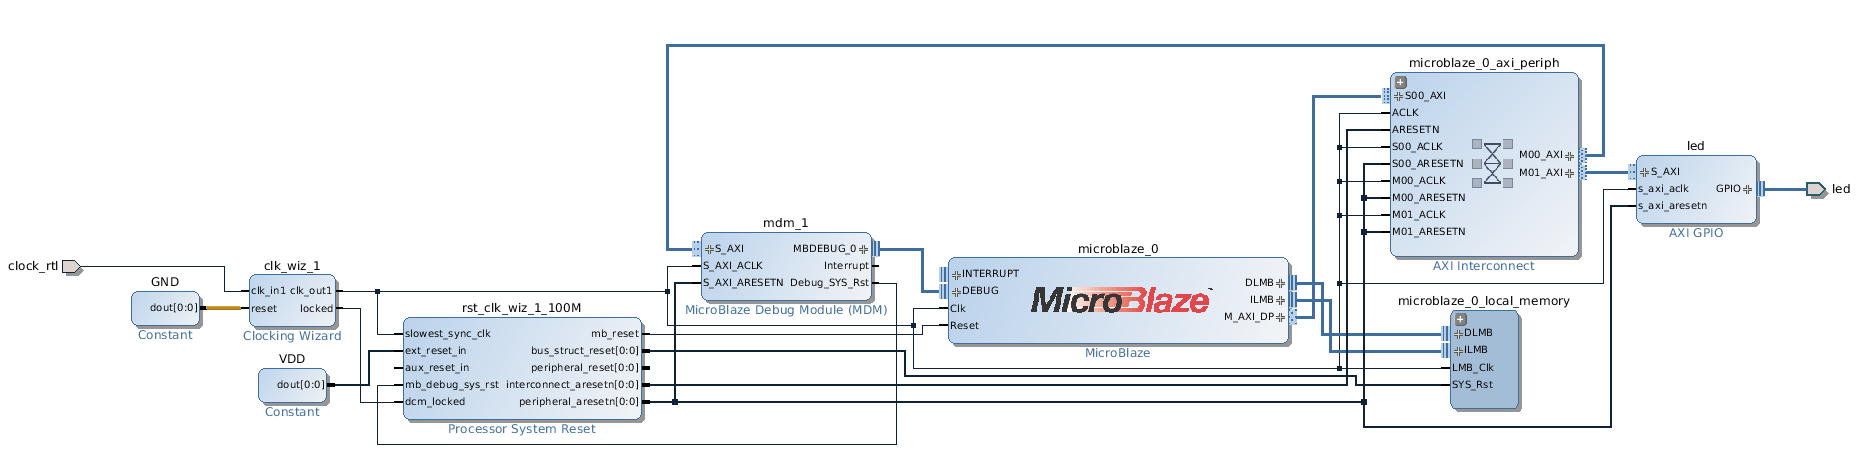
\includegraphics[width=\textwidth]{Ex1_layout.png}
    \caption{Block design for experiment 1.}
    \end{figure}
    
    \item Add the \textit{xdc} constraint file to the design. The file is available on eCampus.
    
    \item Validate design. 
    
    \item Create HDL wrapper. 
    
    \item Generate bitstream.
    
    \item Export the hardware design, including the bitstream.
    
    \item Launch SDK. Create an empty \textbf{Application Project}. Add the source code written in C, available on eCampus, to the project.
    
    \item Program FPGA using SDK and run the C program. Create a new run configuration that uses the \textbf{JTAG UART} port before running the program.
 
\end{enumerate}

\newpage

\section{GPIO Operations with Console Log}

\begin{enumerate}
    \item Create a Vivado project with the same hardware design from experiment 1.
    
    \item In the block diagram editor, add a new GPIO IP block with 8-bit width inputs. Rename the block to \textbf{sw\_buttons}.
    
    \begin{figure}[ht]
    \centering
    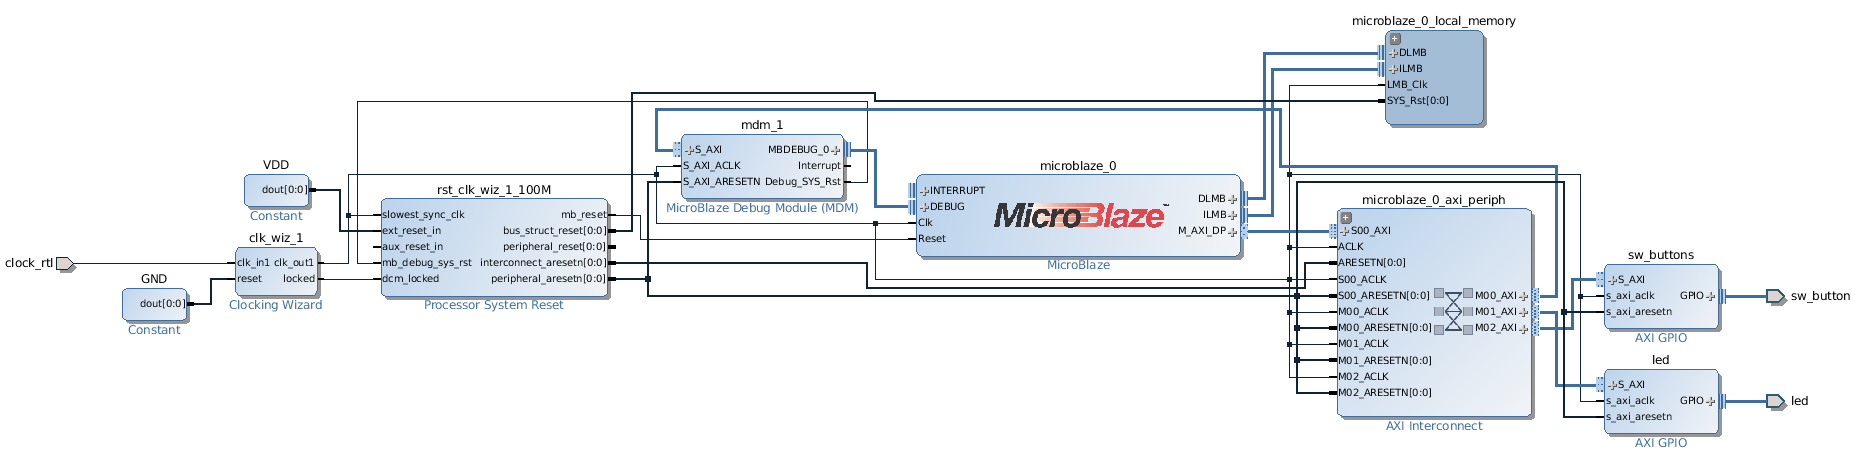
\includegraphics[width=\textwidth]{Ex2_layout.png}
    \caption{Block design for experiment 1.}
    \end{figure}
    
    \item Run connection automation.
    
    \item Run regenerate layout to make the block design look neater.
    
    \item Add the \textit{xdc} constraint file available in \textbf{Appendix} \ref{appendix:GPIO_xdc} to the design project. The constraint is written based on the GPIO blocks imported to the block design and the schematics of the board.
    
    \item Repeat the procedures for generating HDL wrapper and bitstream. 
    
    \item Export the hardware design, including the bitstream.
    
    \item Launch Xilinx SDK and create a new \textbf{Application Project}.
    
    \item Add the code in \textbf{Appendix} \ref{appendix:GPIO_c} to the application project in SDK. If unsure about the name of the variables used in C code, refer to \textbf{xparameter.h}. If unsure about the function to use for reading button and switch status, refer to \textbf{xgpio.h}.
    
    \item Program FPGA and run the code. 
    
\end{enumerate}

\newpage

\part{Results}

\section{LED Counter with Console Log}

The LEDs count from 0 to 15 at an increment speed of approximately 1 second. The console logs the current LED state in hex-decimal format.

\begin{figure}[h!]
\centering
    \begin{subfigure}{0.49\textwidth}
        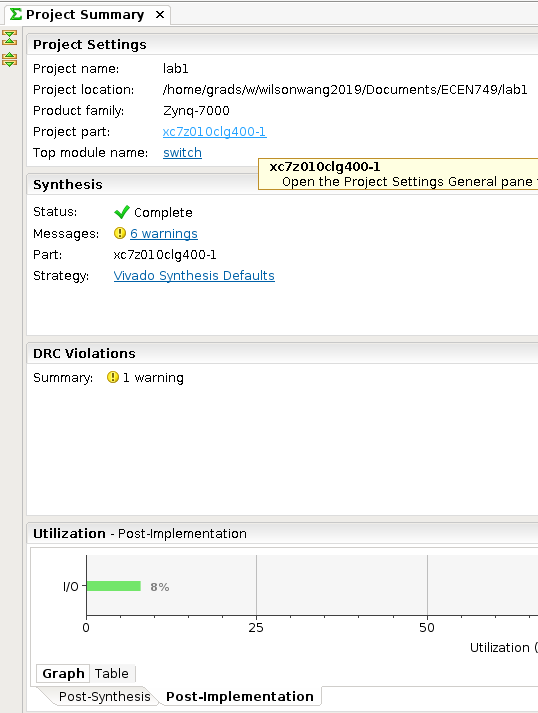
\includegraphics[width=\linewidth]{Lab1_Hardware_Usage.png} 
        \caption{Lab 1 LED counter experiment hardware usage.}
    \end{subfigure}
    \begin{subfigure}{0.49\textwidth}
        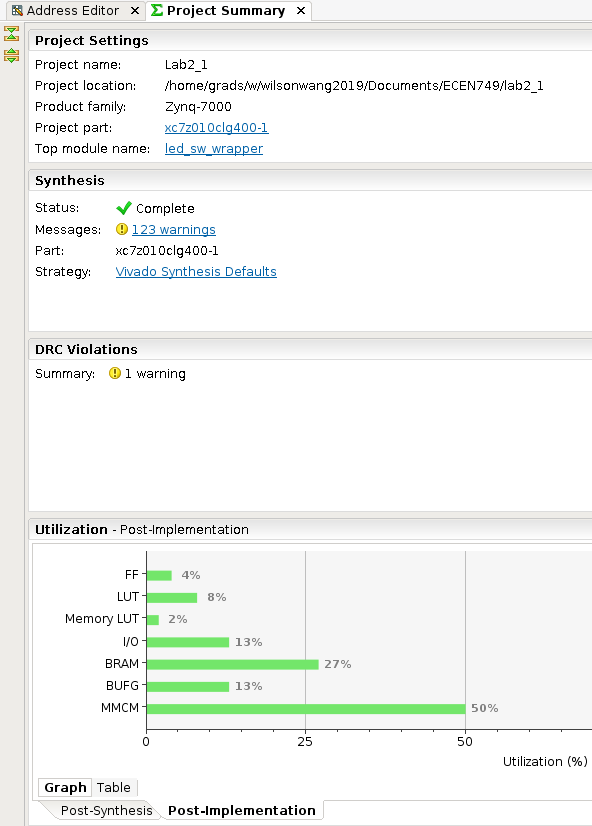
\includegraphics[width=\linewidth]{Lab2_Hardware_Usage.png}
        \caption{Lab 2 LED counter experiment hardware usage.}
    \end{subfigure}
    \caption{Lab 1 and 2 LED counter experiment hardware usage comparison.}
    \label{hardware_comparison}
\end{figure}

As we can see from Figure \ref{hardware_comparison}, a software approach uses much more hardware resource compared with a hardware approach when trying to do the LED counter example.

\newpage

\section{GPIO Operations with Console Log}

The system operates as expected. When pressing button 0, the count value increases at approximately 1Hz. When pressing button 1, the count value decreases at approximately 1Hz. To display switch status in the terminal, press button 2. To display the count value on LEDs, press button 3.

\begin{figure}[ht]
\centering
    \begin{subfigure}[]{0.45\textwidth}
        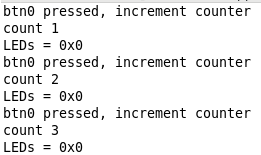
\includegraphics[width=\linewidth]{Btn0.png} 
        \caption{Console output for button 0.}
    \end{subfigure}
    \begin{subfigure}[]{0.45\textwidth}
        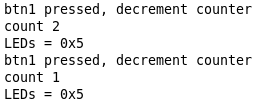
\includegraphics[width=\linewidth]{Btn1.png}
        \caption{Console output for button 1.}
    \end{subfigure}
    \begin{subfigure}[]{0.45\textwidth}
        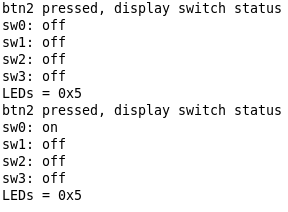
\includegraphics[width=\linewidth]{Btn2.png} 
        \caption{Console output for button 2.}
    \end{subfigure}
    \begin{subfigure}[]{0.45\textwidth}
        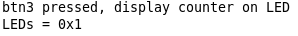
\includegraphics[width=\linewidth]{Btn3.png}
        \caption{Console output for button 3.}
    \end{subfigure}
    \caption{Corresponding console output for pressing buttons.}
\end{figure}

When any of the buttons are pressed, the corresponding action is printed in the terminal as well as the LED value.

\newpage

\part{Conclusion}

To add support for peripheral devices such as buttons and switches, first refer to the schematics of the board to find out the port number. Then add the port number to the \textit{xdc} constraint file. The name of the port, not port number, should be consistent with the name of the block, i.e. the GPIO block, used in the block design editor. Those names will show up in the \textbf{xparameter.h} file after the HDL wrapper, the bitstream and the hardware has been created and exported.

In the example of LED counter, a software approach that needs a MicroBlaze soft processor may need much more hardware resource compared with a direct hardware implementation using Verilog.

\textbf{Q: In the first part of the lab, we created a delay function by implementing a counter. The goal was to update the LEDs approximately every second as we did in the previous lab. Compare the count value in this lab to the count value you used as a delay in the previous lab. If they are different, explain why? Can you determine approximately how many clock cycles are required to execute one iteration of the delay for-loop? If so, how many?}

A: The count value used in the delay function in this lab is 10,000,000 as in the previous lab, the number is 125,000,000. The value used in this lab is smaller. In the previous lab, the count value is the same as the system clock frequency as the hardware is designed to do something per clock cycle. While in this lab, there is one intermediate layer, the MicroBlaze processor. The lines of code that increment the count value do not take exactly one clock cycle to run. Based on the ratio of $ 125000000/10000000 = 12.5 $, approximately 12 or 13 clock cycles are required to execute one iteration of the delay loop.

\textbf{Q: Why is the count variable in our software delay declared as volatile?}

A: To prevent optimization by the compiler. The count variable is forced to to initialize to zero and do the increment process every time the program calls the delay function. In the case of compiler optimization, the count variable may stay at its maximum value and do not increment every time the program calls the delay function.

\textbf{Q: What does the while(1) expression in our code do?}

A: It is an infinite loop that executes the code in the loop infinitely many times until the program is terminated by the user or due to exceptions. We place our code, i.e. increment the counter, display the counter value on LED and print counter value in the terminal, or as described in the second part of the lab, for handling switch and button events, in the infinite loop.

\textbf{Q: Compare and contrast this lab with the previous lab. Which implementation do you feel is easier? What are the advantages and disadvantages associated with a purely software implementation such as this when compared to a purely hardware implementation such as the previous lab?}

A: The implementation in this lab feels easier. The advantages of using software approach is the rich library ecosystem available to use, though Verilog does have libraries, C libraries are much easier to use for a person like me who has some experience with coding but not so much with hardware design. The logic behind C programming is sequential while in Verilog, parallel operations can exist, which makes it difficult to understand and debug. Verilog does not have data types like int or char but pure bytes. Coding in pure bytes instead of meaningful data types can be difficult to understand intuitively.

The disadvantage of using purely software approach is such approach relies on a mature processor system such as the MicroBlaze soft processor running on FPGA. Without such processor, a purely software implementation is impossible as it lacks the ability to communicate with the hardware. A software approach can consume a significant chunk of the hardware resource available on the FPGA board, even the software is very simple and does not require a powerful processor to run. A purely hardware approach can reduce the resource usage since it does not require a complicated soft processor. Since a software approach needs a processor, the setup process can be prone to errors compared with a hardware approach, which involves fewer steps to setup and run.

\newpage

\begin{appendices}

\section{GPIO\_op.xdc}
\label{appendix:GPIO_xdc}
\lstinputlisting[style={txt-style}]{GPIO_op_xdc.txt}

\section{GPIO\_op.c}
\label{appendix:GPIO_c}
\lstinputlisting[style={C-style}]{GPIO_op.c}

\end{appendices}

\end{document}
